
%%%%%%%%%%%%%%%%%%%%%%%%%%%%%%%%%%%%%%%%%%%%%%%%%%%%%%%%%%%%%%%%%%%%%%%%%%%%%%%
% Author:  Pablo Alvarado
%
% Escuela de Ingeniería Electrónica
% Instituto Tecnológico de Costa Rica
%
% Tesis de Licenciatura
% 
% Phone:   +506 2550 9005
% email:   palvarado@itcr.ac.cr
%
%%%%%%%%%%%%%%%%%%%%%%%%%%%%%%%%%%%%%%%%%%%%%%%%%%%%%%%%%%%%%%%%%%%%%%%%%%%%%%%

% \documentclass is book
% If you want a printable two-side version of the thesis
%\documentclass[12pt,twoside,letterpaper]{book}

% If you want an electronic-only version of the thesis, do it one-sided
\documentclass[12pt,oneside,letterpaper]{book}

\usepackage[utf8]{inputenc}
\usepackage{ifthen}       % provide if-then-else operators

\usepackage[backend=bibtex]{biblatex}
\addbibresource{body/literatura.bib}
%\addbibresource{literatura.bib}z
% --------------------------------------------------------------------------
% Global variables required in document formatting
% --------------------------------------------------------------------------
%
% BOOK MODE
%
\newboolean{bookmode}                  % boolean used to control book format
% Ensure that only one of the next two lines is active:
\setboolean{bookmode}{true}           % turn book mode on
%\setboolean{bookmode}{false}           % turn book mode off

%
% DRAFT MODE
%   The draft mode activates the TODO index and some "draft" markings all
%   around.  Ensure you set it to false for the final version!!
%
\newboolean{draftmode}                  % boolean used to control draft-mode
% Ensure that only one of the next two lines is active:
\setboolean{draftmode}{true}            % turn draft mode on
%\setboolean{draftmode}{false}           % turn draft mode off
% --------------------------------------------------------------------------
%
% GENERAL AUTHOR, TITLE AND KEYWORDS
%
% Nombre del Estudiante
\newcommand{\thesisAuthorAddress}{el señor} %% el señor / la señora / ...
\newcommand{\thesisAuthor}{Luis Diego Sandí Quesada} %% Nombre completo
\newcommand{\thesisAuthorShort}{L.~Sandí}  %% Nombre corto para pie de página
\newcommand{\thesisAuthorTECID}{2017098994} %% Carné

% Título de la tesis
\newcommand{\thesisTitle}{Implementación de prueba de concepto de arquitectura de lógica reconfigurable sobre FPGA}

% Keywords
\newcommand{\thesisKeywords}{palabras, clave, ...}

% Tipo de tesis o informe
%   - Tesis de Licenciatura
%   - Informe de Proyecto Final 
%   - Tesis de Maestría
\newcommand{\thesisType}{Tesis de Licenciatura}

% Descripción de la editorial
\newcommand{\boxeditorial}{%
}

% Para el PDF (cambiar si se desea otras cosas a lo indicado arriba
\newcommand{\pdfAuthor}{\thesisAuthor}
\newcommand{\pdfTitle}{\thesisTitle} 
\newcommand{\pdfKeywords}{\thesisKeywords}
\newcommand{\pdfSubject}{\thesisType}
% --------------------------------------------------------------------------

% include all packages and define all required general macros
%%%%%%%%%%%%%%%%%%%%%%%%%%%%%%%%%%%%%%%%%%%%%%%%%%%%%%%%%%%%%%%%%%%%%%%%%%%%%%%
% Author:  Pablo Alvarado
%
% Escuela de Electrónica
% Instituto Tecnológico de Costa Rica
%
% Phone:   +506 2550 9005
% email:   palvarado@itcr.ac.cr
%%%%%%%%%%%%%%%%%%%%%%%%%%%%%%%%%%%%%%%%%%%%%%%%%%%%%%%%%%%%%%%%%%%%%%%%%%%%%%%

% Configuration of the exercises package, which is used to collect all
% problems and answers in the document.
\usepackage[exercisedelayed,answerdelayed,lastexercise]{exercise}
\renewcounter{Exercise}[chapter]
\renewcommand{\ExerciseName}{Problema}
\renewcommand{\theExercise}{\thechapter.\arabic{Exercise}}
\newcommand{\ExerciseLabel}{Exercise.\theExercise}
\renewcommand{\ExerciseHeader}%
{\textbf{\ExerciseName\ \theExercise.\ \ExerciseHeaderTitle\ }}
\renewcommand{\AnswerHeader}%
{\textbf{\ExerciseName\ \theExercise.\ }}


\usepackage{ifpdf}

% Command to change between draft or release mode:
\newcommand{\ifdraft}[2]{\ifthenelse{\boolean{draftmode}}{#1}{#2}}
% Command to change between draft or release mode:
\newcommand{\ifbook}[2]{\ifthenelse{\boolean{bookmode}}{#1}{#2}}

% include all required packages here
\usepackage{csquotes}                     % recommended for biblatex
\usepackage[spanish]{babel}               % supports english, but default is 
                                          % spanish...
% \newcommand*{\SelectSpanish}{%          % well, the last line indeed selects
%   \hyphenrules{spanish}%                % english over spanish, but with this
%   \languageshorthands{spanish}%         % command we turn it around.
%   \captionsspanish                      % The reason: hyperref has some
%   \datespanish                          % problems with the spanish babel,
% }                                       % so we use some trick here so that it
% \AtBeginDocument{\SelectSpanish}        % thinks it is english.

\usepackage{makeidx}                    % to create index file

\usepackage[nottoc]{tocbibind}          % Fix the hyperrefs to TOC,TOF, etc.
                                        % and ensure that they appear all in 
                                        % the Table of Contents
\ifdraft{%
  %\usepackage[refpage]{nomencl}        % Use to easily administrate the list
  \usepackage[intoc,spanish]{nomencl}    % of symbols
}{%
  \usepackage[intoc,spanish]{nomencl}
}
%\usepackage{times}                     % replace latex pk fonts with ps type I
                                        % don't forget to use dvips -D600 -Pcmz
                                        % to ensure Type I fonts!
\usepackage{siunitx}                    % Units of the SI
\sisetup{output-decimal-marker = {,}}
\DeclareSIQualifier\peak{p}
\DeclareSIQualifier\ppeak{pp}

\usepackage{amsmath}
\usepackage{amssymb,amstext}            % AMS-math and symbols package
\usepackage{mathrsfs}                   % Calygraphic fonts for transforms
\usepackage{trsym}                      % Para símbolos de transformadas o---o
\usepackage{stmaryrd}                   % For short arrows
\usepackage{nicefrac}
\usepackage{array}                      % extensions to tabular environment
\usepackage{longtable}                  % supports extraordinary long tables
\usepackage{tabularx}                   % supports tables with fixed width

\usepackage{afterpage}                  % put something only after the page
\usepackage{multirow}                   % supports multiple row grouping in 
                                        % tables
\usepackage{multicol}                   % multiple columns environments
\usepackage{enumitem}                   % better enumeration with paralist 
                                        % equivalents as follows:

\newlist{compactitem}{itemize}{3}
\setlist[compactitem]{topsep=0pt,partopsep=0pt,itemsep=0pt,parsep=0pt}
\setlist[compactitem,1]{label=\textbullet}
\setlist[compactitem,2]{label=---}
\setlist[compactitem,3]{label=*}

\newlist{compactdesc}{description}{3}
\setlist[compactdesc]{topsep=0pt,partopsep=0pt,itemsep=0pt,parsep=0pt}

\newlist{compactenum}{enumerate}{3}
\setlist[compactenum]{label*=\arabic*.,topsep=0pt,partopsep=0pt,itemsep=0pt,parsep=0pt}
\newlist{compactenuma}{enumerate}{3}
\setlist[compactenuma]{label*=\alph*.,topsep=0pt,partopsep=0pt,itemsep=0pt,parsep=0pt}

\usepackage{icomma}                     % decimal comma in math mode

\usepackage{bold-extra}

\usepackage[format=hang,%
            font=small,%
            labelfont=bf]{caption}      % nicer figure captions
% locally added packages
\usepackage{float}                      % really place figures "here" (H)
\usepackage{booktabs}                   % book type tabulars

% the own style with options depending on the draft mode
\ifdraft{%
\usepackage[todo]{sty/tecStyle}         % some command definitions
                                        % options [todo] todo-index
}{%
\usepackage{sty/tecStyle}               % some command definitions
                                        % options [todo] todo-index
}

%% fix the title for examples
\renewcommand{\examplelistname}{Índice de ejemplos}
\renewcommand{\examplename}{Ejemplo}

%% define some command to cope with the tribunal names

%% Lector I

\newcommand{\nameLectorI}{$<$\emph{Use setLectorI in main.tex}$>$}
\newcommand{\genderLectorI}{$<$\emph{Use setLectorI in main.tex}$>$}

\newcommand{\setLectorI}[1][M]{%
  \ifthenelse{\equal{#1}{F}}{%
    \renewcommand{\genderLectorI}{Profesora Lectora}%
  }{%
    \renewcommand{\genderLectorI}{Profesor Lector}
  }
  \lectorIRelay
}

\newcommand{\lectorIRelay}[1]{%
  \renewcommand{\nameLectorI}{#1}
}

%% Lector II

\newcommand{\nameLectorII}{$<$\emph{Use setLectorII in main.tex}$>$}
\newcommand{\genderLectorII}{$<$\emph{Use setLectorII in main.tex}$>$}

\newcommand{\setLectorII}[1][M]{%
  \ifthenelse{\equal{#1}{F}}{%
    \renewcommand{\genderLectorII}{Profesora Lectora}%
  }{%
    \renewcommand{\genderLectorII}{Profesor Lector}
  }
  \lectorIIRelay
}

\newcommand{\lectorIIRelay}[1]{%
  \renewcommand{\nameLectorII}{#1}
}

%% Asesor

\newcommand{\nameAsesor}{$<$\emph{Use setAsesor in main.tex}$>$}
\newcommand{\genderAsesor}{$<$\emph{Use setAsesor in main.tex}$>$}

\newcommand{\setAsesor}[1][M]{%
  \ifthenelse{\equal{#1}{F}}{%
    \renewcommand{\genderAsesor}{Profesor Asesor}%
  }{%
    \renewcommand{\genderAsesor}{Profesor Asesor}
  }
  \asesorRelay
}

\newcommand{\asesorRelay}[1]{%
  \renewcommand{\nameAsesor}{#1}
}

\usepackage{url}                        % allows linebreaks at certain
                                        % characters or combinations of 
                                        % characters for URLs

% For pdflatex
% - The hyperref package should always be loaded last, since it has to
%   overwrite some of the commands.
% - The package subfigure caused that the pagebackrefs and index refs were set
%   incorrectly.

\ifpdf
%
% final / draft document options
%\usepackage{graphicx}                   % for inserting pdf-graphics.
                                        % options final / draft
\ifdraft{%
\usepackage[%pdftex,%
            naturalnames=true,
            linktocpage,
            hyperindex,
            colorlinks,
            urlcolor=dkred,          %\href to external url
            filecolor=dkmagenta,     %\href to local file
            linkcolor=dkred,         %\ref and \pageref
            citecolor=dkgreen,       %\cite
            plainpages=false,
            pdfpagelabels,
            pdfpagemode=UseOutlines, % means use bookmarks (None,UseOutlines)
            % bookmarksopen=false,   % would show the whole hierarchy if true
            bookmarksnumbered=true,
            pdfpagelayout=OneColumn, % SinglePage,OneColumn,TwoColumnLeft,...
            pdfview=FitH, % FitB,FitBH,FitBV,Fit,FitH,FitV
            pdfstartview=FitH, % FitB,FitBH,FitBV,Fit,FitH,FitV
            ]{hyperref}
}{%
% Use biber/biblatex
\usepackage[%pdftex,%
            naturalnames=true,
            linktocpage,hyperindex,
            colorlinks,
            urlcolor=dkred,          %\href to external url
            filecolor=dkmagenta,     %\href to local file
            linkcolor=dkred,         %\ref and \pageref
            citecolor=dkgreen,       %\cite
            plainpages=false,
            pdfpagelabels,
            pdfpagemode=UseOutlines, % means use bookmarks (None,UseOutlines)
            % bookmarksopen=false,   % open the whole hierarchy if true!
            bookmarksnumbered=true,
            pdfpagelayout=OneColumn, % SinglePage,OneColumn,TwoColumnLeft,...
            pdfview=FitH, % FitB,FitBH,FitBV,Fit,FitH,FitV
            pdfstartview=FitH, % FitB,FitBH,FitBV,Fit,FitH,FitV
            ]{hyperref}
}


%
% Ensure that the links of the images point to the top of the images and not
% to the caption
%
\usepackage[figure]{hypcap}

% %
% % Ensure that pdfLaTeX do the same spacing as LaTeX
% %
\pdfadjustspacing=1 
% %
\else   % i.e. if not pdf

\usepackage[active]{srcltx}             % insert links into the dvi to jump
\usepackage{graphicx}                   % for inserting eps-graphics.
                                        % options final / draft
                                        % into the sources directly.
\ifdraft{%
\usepackage[ps2pdf,%
            % plainpages=false,
            linktocpage,
            hyperindex,
            % pdfpagelabels,
            pdfpagemode=UseOutlines,
            pdfstartview=FitH]{hyperref}
}{%
\usepackage[ps2pdf,%
            % plainpages=false,
            linktocpage,
            hyperindex,
            % pdfpagelabels,
            pdfpagemode=UseOutlines,
            pdfstartview=FitH]{hyperref}
}

%\usepackage[ps2pdf]{hyperref}

\fi  % end of if pdf or not

% --------------------------------------------------------------------------

% Allow the use of international characters
\AtBeginDocument{%
  \hypersetup{%
             pdftitle={\pdfTitle},%
             pdfsubject={\pdfSubject},%
             pdfauthor={\pdfAuthor},%
             pdfkeywords={\pdfKeywords}
            }%
}


%\usepackage{algorithmic}            % algorithmic environment


\usepackage{rotating}                % allow block rotation


%%%%%%%%%%%%%%%%%%%%%%%%%%%%%%%%%%%%%%%%%%%%%%%%%%%%%%%%%%%%%%%%%%%%%%%%%%%%%%%

%\sloppy

%
% Some own font definitions
%
\DeclareMathAlphabet{\mathpzc}{OT1}{pzc}{m}{it}
\DeclareMathAlphabet{\mathpss}{OT1}{cmss}{m}{sl}

%
% page layout
%

\usepackage{vmargin}
\setpapersize{USletter}

% For letter-paper printing
\setmarginsrb{33mm}{8mm}{23mm}{7mm}{15pt}{15pt}{7mm}{12mm}
%\setlength{\headheight}{15pt}         % fancy headers wanted this

%
% Fraction of Float Object / Text
%

\renewcommand{\topfraction}{0.95}       % how much of top of page should be 
                                        % allowed to be float object?
\renewcommand{\bottomfraction}{0.95}    % how much of bottom of page should be
                                        % allowed to be float object?
\renewcommand{\textfraction}{0.05}      % how much of page must be text?

\usepackage{fancyhdr}                   % fancy page headers

\usepackage{lastpage}

%
% header and footer layout (needs package fancyhdr)
%
\newcommand{\copyrightfooter}{\tiny{\copyright \the\year\ --- \thesisAuthorShort %
    \qquad Uso exclusivo ITCR}}
%
\newcommand{\draftfoot}%
  {\ifdraft{\textcolor{dkblue}{\tiny\textsl{Borrador: \today}}{}}
           {}
}

\pagestyle{fancy}
\renewcommand{\chaptermark}[1]{\markboth{{\small
    \thechapter\hspace*{1mm}#1}}{}}
\renewcommand{\sectionmark}[1]{\markright{{\small
    \thesection\hspace*{1mm}#1}}{}}
%\lhead[{\small\textsc\Roman{\thepage}}]{\fancyplain{}%
\lhead[{\small\thepage}]{\fancyplain{}%
        {{\slshape \small\nouppercase{\leftmark}}}}
\chead[]{}
\rhead[\fancyplain{}%
%        {{\slshape \small\nouppercase{\rightmark}}}]{{\small\textsc\Roman{\thepage}}}
        {{\slshape \small\nouppercase{\rightmark}}}]{{\small\thepage}}
\lfoot[]{\draftfoot}
\ifbook{%
  \cfoot[]{}
}{
  \cfoot[\copyrightfooter]{\copyrightfooter}
}
\rfoot[\draftfoot]{}
\renewcommand{\headrulewidth}{0.5pt}
\renewcommand{\footrulewidth}{0pt}

%
% Caption style for tables
% For caption v3:
\captionsetup[table]{position=top,
  format=hang,
  textfont={normalsize},
  labelfont={normalsize,bf}}

\newcommand{\tablecaption}[2][foo]{%
  \ifthenelse{\equal{#1}{foo}}{%
    %\captionstyle{tablecaptionstyle}%
    \caption{#2}%
  }
  {%
    %\captionstyle{tablecaptionstyle}%
    \caption[#1]{#2}%
  }
}
\addto\extrasspanish{\renewcommand{\tablename}{Tabla}}
\addto\extrasspanish{\renewcommand{\listtablename}{\'Indice de tablas}}

%
% paragraph layout
%
\renewcommand{\baselinestretch}{1.1}    % line spacing
\parindent0em                           % indentation width of first line
\parskip1.3ex                           % space between paragraphs

%
% document consists of
% chapter - section - subsection - subsubsection - paragraph - subparagraph
%
\setcounter{secnumdepth}{2}             % depth of section numbering
\setcounter{tocdepth}{2}                % depth of table of contents

%
% prepares index from entries like \index{word} or \index{group!word}.
% don't forget to call "makeindex filename" for final index generation.
%
\makeindex                            %% for package makeidx.sty
%\newindex{default}{idx}{ind}{Index}  %% for package index.sty

\newcommand{\octave}{GNU/Octave}


%
% prepares notation or nomenclature 
%
\makenomenclature

%%% Local Variables: 
%%% mode: latex
%%% TeX-master: "main"
%%% End: 


% Tribunal Evaluador
%
% Indique los nombres de los lectores y asesor
% El parámetro opcional es [M]asculino o [F]emenino

\setLectorI[F]{M.Sc.\,Por definir}
\setLectorII{M.Sc.\,Por definir}
\setAsesor{Dr. -Ing\, Pablo Mendoza Ponce}

% allow equations to be splitted (breaked) into several pages
\allowdisplaybreaks[3]

% --------------------------------------------------------------------------
\begin{document}
  % where to look for graphics
    \graphicspath{{./}{./fig/}}

    \pagenumbering{alph}
  % fix some terms not activated due to the bug of hyperref with spanish.
  \renewcommand{\tablename}{Tabla}
  \renewcommand{\listtablename}{Índice de tablas}
  \renewcommand{\examplesolution}{Solución}
  \pagestyle{empty}

  % select one of the following titlepages
  
  %% ---------------------------------------------------------------------------
%% titlepage_licce_es.tex
%%
%% Title page
%%
%% $Id: titlepage.tex 1452 2010-07-07 00:55:16Z palvarado $
%% ---------------------------------------------------------------------------

\thispagestyle{empty} 

\begin{center}

Tecnológico de Costa Rica

\par\vspace{1ex}

Escuela de Ingeniería Electrónica

\par\vspace{1ex}

Programa de Licenciatura en Ingeniería Electrónica

\par\vspace{20mm}


\includegraphics[width=60mm]{pics/Firma_TEC-4.pdf}

\par\vspace*{\fill}

{\large\bf{\thesisTitle}}

\par\vspace*{\fill}

Informe de Ante Proyecto de Graduación para optar por el título de

Ingeniero en Electrónica con el grado académico de Licenciatura

\par\vspace{20mm}

\thesisAuthor 

Asesor: Dr.\, Pablo Mendoza Ponce

Campus Central

\vspace*{\fill}

\ifdraft{%
{ \today}
}{
Cartago,  de abril, 2023
}
\end{center}
\newpage 
\cleardoublepage 


%%% Local Variables: 
%%% mode: latex
%%% TeX-master: "main"
%%% End: 
 % Titlepage in Spanish
  \thispagestyle{empty}

\rule{10mm}{0pt}

\vfill

Declaro que el presente documento de tesis ha sido realizado enteramente
por mi persona, utilizando y aplicando literatura referente al tema e
introduciendo conocimientos y resultados experimentales propios.

En los casos en que he utilizado bibliografía he procedido a indicar las
fuentes mediante las respectivas citas bibliográficas.  En consecuencia,
asumo la responsabilidad total por el trabajo de tesis realizado y por
el contenido del presente documento.



\vspace*{8mm}

\begin{flushright}
  \thesisAuthor\par
  Cartago, \today\par
  Céd: 1-1750-0693
\end{flushright}

\cleardoublepage

%%% Local Variables: 
%%% mode: latex
%%% TeX-master: "main"
%%% End: 

  
  %% -------------------------------------------------
  
  %% Para la licenciatura en electrónica:
  %% ESTE ARCHIVO DEBE ELIMINARSE DE LA VERSIÓN FINAL

\thispagestyle{empty}

\begin{center}
  \begin{tabular}{c}
    Instituto Tecnológico de Costa Rica \\
    Escuela de Ingeniería Electrónica \\
    Ante Proyecto de Graduación \\
    Acta de Aprobación
  \end{tabular}
\end{center}

\vfill

\begin{center}
  \begin{tabular}{c}
    Defensa de Proyecto de Graduación \\
    Requisito para optar por el título de Ingeniero en Electrónica \\
    Grado Académico de Licenciatura
  \end{tabular}
\end{center}

\vfill

%% \thesisAuthorAddress, \thesisAuthor y \thesisTitle están en main.tex
El Tribunal Evaluador aprueba la defensa del proyecto de graduación
denominado \textsl{\thesisTitle}, realizado por
%
\thesisAuthorAddress\ \thesisAuthor\ %
%
y, hace constar que cumple con las normas
establecidas por la Escuela de Ingeniería Electrónica del Instituto
Tecnológico de Costa Rica.

\vfill

\begin{center}
 Miembros del Tribunal Evaluador
\end{center}

\vfill

\begin{center}
  \begin{tabularx}{\textwidth}{cXc}
    \rule{0.45\textwidth}{0.5pt} && \rule{0.45\textwidth}{0.5pt} \\
    \nameLectorI                 && \nameLectorII \\
    \genderLectorII               && \genderLectorII
  \end{tabularx}
  
  \vspace{10mm}

  \begin{tabular}{c}
    \rule{0.45\textwidth}{0.5pt} \\
    \nameAsesor \\
    \genderAsesor
  \end{tabular}
\end{center}

\vfill

\begin{center}
  Cartago, \today\par
\end{center}

\cleardoublepage

%%% Local Variables: 
%%% mode: latex
%%% TeX-master: "main"
%%% End: 
  % Remover en versión final
  %% ESTE ARCHIVO DEBE ELIMINARSE DE LA VERSIÓN FINAL


\thispagestyle{empty}

\begin{center}
  \begin{tabular}{c}
    Instituto Tecnológico de Costa Rica \\
    Escuela de Ingeniería Electrónica \\
    Proyecto de Graduación \\
    Tribunal Evaluador \\
    Acta de Evaluación
  \end{tabular}
\end{center}

\vfill

\begin{center}
  \begin{tabular}{c}
    Defensa de Proyecto de Graduación \\
    Requisito para optar por el título de Ingeniero en Electrónica \\
    Grado Académico de Licenciatura
  \end{tabular}
\end{center}

\vfill

%% \thesisAuthorAddress, \thesisAuthor y \thesisTitle están en main.tex
\begin{center}

  Estudiante:%
  \qquad \textbf{\thesisAuthor}%
  \qquad Carné: \thesisAuthorTECID

  \vspace*{2ex}

  \setlength\tabcolsep{0pt}
  \begin{tabular}{p{.25\textwidth}p{.73\textwidth}}
    Nombre del proyecto: & \textsl{\thesisTitle}
  \end{tabular}
\end{center}
\vspace{5mm}

\vfill

Los miembros de este Tribunal hacen constar que este proyecto de
graduación ha sido aprobado y cumple con las normas establecidas por
la Escuela de Ingeniería Electrónica del Instituto Tecnológico de
Costa Rica y es merecedor de la siguiente calificación:

\vfill

\begin{center}
  Nota de Proyecto de Graduación: \rule{25mm}{0.5pt}
\end{center}

\vfill

\begin{center}
 Miembros del Tribunal Evaluador
\end{center}

\vfill

% Defina con \setLector* en main.tex (líneas 87-89) los lectores y asesor
\begin{center}
  \begin{tabularx}{\textwidth}{cXc}
    \rule{0.45\textwidth}{0.5pt} && \rule{0.45\textwidth}{0.5pt} \\
    \nameLectorI                 && \nameLectorII \\
    \genderLectorII               && \genderLectorII
  \end{tabularx}
  
  \vspace{10mm}

  \begin{tabular}{c}
    \rule{0.45\textwidth}{0.5pt} \\
    \nameAsesor \\
    \genderAsesor
  \end{tabular}
\end{center}

\vfill

\begin{center}
  Cartago, \today\par
\end{center}

\cleardoublepage

%%% Local Variables: 
%%% mode: latex
%%% TeX-master: "main"
%%% End: 
      % Remover en versión final
  
  %% Para la maestría en electrónica:
  %\include{tribunal_mscel}  % Remover en versión final
  %\include{acta_mscel}      % Remover en versión final
  
  %% -------------------------------------------------
  
  %\chapter*{Resumen}
\thispagestyle{empty}



\bigskip

\textbf{Palabras clave: } FPGA, LUTs, Matriz de conmutación, Validación, Testeo, JTAG, TAP, Lógica Reconfigurable.

%\clearpage
%\chapter*{Abstract}
%\thispagestyle{empty}


%\bigskip

%\textbf{Keywords:}  Intel, Microprocessors, Xeon, Validation, Testing, PPV, Bucket, Debug, Sequential Algorithm, Search Algorithm.

%\cleardoublepage

%%% Local Variables: 
%%% mode: latex
%%% TeX-master: "main"
%%% End: 

  %\chapter*{Dedicatoria}
\vspace*{0.4\textheight}
{\hfill{\Large{\emph{A todos aquellos que han sido una parte integral de mi camino académico y personal. A mis padres, por su amor incondicional y por creer en mí desde el primer día. Por sus sacrificios y su apoyo constante que han sido la clave de mi éxito. A mis profesores y mentores, por su dedicación y pasión por la enseñanza y por guiarme en mi camino.  }}}}

  %\chapter*{Agradecimientos}
\thispagestyle{empty}

El resultado de este trabajo no hubiese sido posible sin el apoyo de Componentes Intel de Costa Rica, por suministrarme los datos y herramientas para la elaboración del proyecto así como mi ..\par
Asimismo, quiero agradecer a mi profesor asesor ..., quien me guió en todo el transcurso de este proyecto.\par

\vspace*{1cm}

\thesisAuthor

Cartago, \today

\cleardoublepage

%%% Local Variables: 
%%% mode: latex
%%% TeX-master: "paMain"
%%% End: 


  %----------------------------------------------------------------------------
  \pagestyle{fancy}
  \pagenumbering{roman}

  \pdfbookmark[1]{Indice General}{Indice General}

  \parskip0ex                           % space between paragraphs

  \tableofcontents                      % Table of contents
  \listoffigures                        % List of figures
  \listoftables                         % List of tables



  %% ---------------------------------------------------------------------------
%% paNotation.tex
%%
%% Notation
%%
%% $Id: notation.tex 1467 2010-07-24 16:47:17Z palvarado $
%% ---------------------------------------------------------------------------

\newcommand{\nms}{\negmedspace}

%%
% Commands required for the nomenclature groups
%
% There are following prefix forms:
%  a   abbreviation    \syma[key]{symbol}{description}
%  g   general         \symg[key]{symbol}{description}
%%

\newcommand{\nmstyle}[1]{\large\item[\textbf{#1}]\normalsize}

\renewcommand{\nomgroup}[1]{%
  \ifthenelse{\equal{#1}{A}}{\nmstyle{Abreviaciones}\normalsize}{%
  \ifthenelse{\equal{#1}{G}}{\bigskip\nmstyle{Notación general}\normalsize}%
  }
}

\newcommand{\syma}[3][foo]{%
  \ifthenelse{\equal{#1}{foo}}%
  {\nomenclature[A#2\ ]{#2}{#3}}{\nomenclature[A#1\ ]{#2}{#3}}}
\newcommand{\symg}[3][foo]{%
  \ifthenelse{\equal{#1}{foo}}%
  {\nomenclature[G#2\ ]{#2}{#3}}{\nomenclature[G#1\ ]{#2}{#3}}}

%%
% Command definitions for localized symbol format definition
%%
\renewcommand{\Re}{\operatorname{Re}}
\renewcommand{\Im}{\operatorname{Im}}

\newcommand{\prt}[1]{\ensuremath{\mathcal{#1}}}         %% partitioning
\newcommand{\img}[1]{\ensuremath{\mathcal{#1}}}         %% image as a set
\newcommand{\reg}[1][R]{\ensuremath{\mathcal{#1}}}      %% region
\newcommand{\pred}[1]{\ensuremath{\mathrm{#1}}}         %% predicate
\newcommand{\operat}[2]{\mathcal{#1}\left\{#2\right\}}
\newcommand{\transf}[1]{\mathscr{#1}}
\newcommand{\fourier}[1]{\transf{F}\left\{#1\right\}}
\newcommand{\ifourier}[1]{\transf{F}^{-1}\left\{#1\right\}}
\newcommand{\laplace}[1]{\transf{L}\left\{#1\right\}}
\newcommand{\ulaplace}[1]{\transf{L}_u\left\{#1\right\}}
\newcommand{\blaplace}[1]{\transf{L}_b\left\{#1\right\}}
\newcommand{\ilaplace}[1]{\transf{L}^{-1}\left\{#1\right\}}
\newcommand{\ztrans}[1]{\transf{Z}\left\{#1\right\}}
\newcommand{\iztrans}[1]{\transf{Z}^{-1}\left\{#1\right\}}
\newcommand{\zutrans}[1]{\transf{Z}_u\left\{#1\right\}}
\newcommand{\exceq}{\ensuremath{\overset{!}{=}}}

\newcommand{\signum}{\operatorname{signum}}
\newcommand{\vct}[1]{\ensuremath{\underline{\mathbf{#1}}}}
\newcommand{\mat}[1]{\ensuremath{\mathbf{#1}}}
\newcommand{\vctmu}{\vct{\boldsymbol{\mu}}}
\newcommand{\vctzeta}{\vct{\boldsymbol{\zeta}}}
\newcommand{\vctpi}{\vct{\boldsymbol{\pi}}}
\newcommand{\vctvarphi}{\vct{\boldsymbol{\varphi}}}
\newcommand{\raum}[1]{\ensuremath{\mathbb{#1}}}
\newcommand{\matSigma}{\mat{\boldsymbol{\Sigma}}}
\newcommand{\matLambda}{\mat{\boldsymbol{\Lambda}}}
\newcommand{\matPsi}{\mat{\boldsymbol{\Psi}}}
\newcommand{\matPhi}{\mat{\boldsymbol{\Phi}}}
\newcommand{\row}[2]{\ensuremath{\mathbf{\underline{#1}_{#2(\cdot)}}}}
\newcommand{\col}[2]{\ensuremath{\mathbf{\underline{#1}_{(\cdot) #2}}}}
\newcommand{\seq}[1]{\ensuremath{#1}}
\newcommand{\set}[1]{\ensuremath{\mathcal{#1}}}
\newcommand{\gset}[1]{\ensuremath{#1}} %% set for greek symbols
\newcommand{\front}[1]{\widehat{\set{#1}}}
\newcommand{\setlambda}{\set{\boldsymbol{\lambda}}}
\newcommand{\klass}[1]{\ensuremath{\mathpss{#1}}}
\newcommand{\graph}[1]{\ensuremath{\mathsf{#1}}}
\newcommand{\lab}[1]{\ensuremath{\mathpss{L}(#1)}}
\newcommand{\myfrac}[2]{{\footnotesize #1/#2}}
\newcommand{\ifthenspc}{\rule{3mm}{0mm}}
\newcommand{\point}[1]{\ensuremath{\mathsf{#1}}}
\newcommand{\estim}[1]{\ensuremath{\hat{#1}}}
\newcommand{\numset}[1]{\ensuremath{\mathbb{#1}}}
\newcommand{\tuple}[1]{\ensuremath{\left\langle#1\right\rangle}}
\newcommand{\norm}[1]{\ensuremath{\left\lVert#1\right\rVert}}
\newcommand{\conj}[1]{\ensuremath{{{#1}^{\ast}}}}
\newcommand{\base}[1]{\set{#1}}
\newcommand{\zeron}[1]{\ensuremath{\underset{\uparrow}{#1}}}
\newcommand{\sysT}{\ensuremath{\mathcal{T}}}
\newcommand{\sys}[1]{\ensuremath{\sysT\left[#1\right]}}
%\newcommand{\sen}{\operatorname{sen}} % sinus in spanish (seno)
%\newcommand{\senh}{\operatorname{senh}} % sinus hiperbolicus in spanish (seno)
%\newcommand{\arcsen}{\operatorname{arcsen}} % arcus sinus hiperbolicus in spanish (arcoseno)
\newcommand{\sgn}{\operatorname{sgn}} % signus
\newcommand{\roc}{\text{ROC: }}

\newcommand{\code}[1]{\texttt{#1}}
\newcommand{\conv}{\ensuremath{\ast}}
\newcommand{\cconv}{\ensuremath{\;\,\text{\footnotesize{N}}\!\!\!\!\!\!\bigcirc}}
\newcommand{\Ln}{\operatorname{Ln}}
\newcommand{\rand}{\operatorname{rand}}
\newcommand{\sa}{\operatorname{sa}}
\newcommand{\senc}{\operatorname{senc}}


%% Natural, Integer and Real Numbers
\newcommand{\setA}{\ensuremath{\mathbb{A}}}
\newcommand{\setB}{\ensuremath{\mathrm{I\negthinspace B}}}
\newcommand{\setC}{\ensuremath{\mathbb{C}}}
\newcommand{\setD}{\ensuremath{\mathrm{I\negthinspace D}}}
\newcommand{\setE}{\ensuremath{\mathrm{I\negthinspace E}}}
\newcommand{\setF}{\ensuremath{\mathrm{I\negthinspace F}}}
\newcommand{\setG}{\ensuremath{\mathbb{G}}}
\newcommand{\setH}{\ensuremath{\mathrm{I\negthinspace H}}}
\newcommand{\setI}{\ensuremath{\mathbb{I}}}
\newcommand{\setJ}{\ensuremath{\mathbb{J}}}
\newcommand{\setK}{\ensuremath{\mathrm{I\negthinspace K}}}
\newcommand{\setL}{\ensuremath{\mathrm{I\negthinspace L}}}
\newcommand{\setM}{\ensuremath{\mathrm{I\negthinspace M}}}
\newcommand{\setN}{\ensuremath{\mathrm{I\negthinspace N}}}
\newcommand{\setO}{\ensuremath{\mathbb{O}}}
\newcommand{\setP}{\ensuremath{\mathrm{I\negthinspace P}}}
\newcommand{\setQ}{\ensuremath{\mathbb{Q}}}
\newcommand{\setR}{\ensuremath{\mathrm{I\negthinspace R}}}
\newcommand{\setS}{\ensuremath{\mathbb{S}}}
\newcommand{\setT}{\ensuremath{\mathbb{T}}}
\newcommand{\setU}{\ensuremath{\mathbb{U}}}
\newcommand{\setV}{\ensuremath{\mathbb{V}}}
\newcommand{\setW}{\ensuremath{\mathbb{W}}}
\newcommand{\setX}{\ensuremath{\mathbb{X}}}
\newcommand{\setY}{\ensuremath{\mathbb{Y}}}
\newcommand{\setZ}{\ensuremath{\mathbb{Z}}}


%%
% Multimap symbols
%
\newcommand{\ttoF}{\,\circ\!\negthickspace\longrightarrow\negthickspace\!\negthickspace\bullet\,}
\newcommand{\Ftot}{\,\bullet\negthickspace\!\negthickspace\longleftarrow\!\negthickspace\circ\,}
\newcommand{\ttoZ}{\ttoF}
\newcommand{\Ztot}{\Ftot}
\newcommand{\ttoZu}{\overset{z_u}{\ttoF}}
\newcommand{\Zutot}{\overset{z_u}{\Ftot}}
\newcommand{\vttoF}{\text{\begin{sideways}$\Ftot$\end{sideways}}}
\newcommand{\vFtot}{\text{\begin{sideways}$\ttoF$\end{sideways}}}
\newcommand{\vttoZ}{\vttoF}
\newcommand{\vZtot}{\vFtot}
\newcommand{\ttoDF}{\underset{N}{\ttoF}}
\newcommand{\DFtot}{\underset{N}{\Ftot}}

\newcommand{\thisis}[2]{\underset{#1}{\underbrace{#2}}}

%%% Local Variables:
%%% mode: latex
%%% TeX-master: "paMain"
%%% End:
                    % Notation
  %% ---------------------------------------------------------------------------
%% paNotation.tex
%%
%% Notation
%%
%% $Id: paNotation.tex,v 1.15 2004/03/30 05:55:59 alvarado Exp $
%% ---------------------------------------------------------------------------

\cleardoublepage
\renewcommand{\nomname}{Lista de símbolos y abreviaciones}
\markboth{\nomname}{\nomname}
\renewcommand{\nompreamble}{\addcontentsline{toc}{chapter}{\nomname}%
\setlength{\nomitemsep}{-\parsep}
\setlength{\itemsep}{10ex}
}

%%
% Algunas abreviaciones
%%

\syma{TP}{Test Program}
\syma{PPV}{Product Platform Validation}
\syma{DTD}{Debug and Test Development}
\syma{DTD}{Debug and Test Development}
\syma{ALU}{Unidad Aritmético-Lógica}
\syma{AVX-512}{Advanced Vector Extensions 512}
\syma{L1}{Caché de Nivel 1}
\syma{L2}{Caché de Nivel 2}
\syma{L3}{Caché de Nivel 3}
\syma{QPI}{QuickPath Interconnect}
\syma{UPI}{Ultra Path Interconnect}
\syma{VT-d}{Virtualization Technology for Directed I/O}
\syma{VT-x}{Virtualization Technology}
\syma{CPU}{Central Processing Unit} 
\syma{Vdd}{Voltage Drain Drain} 
\syma{GHz}{Gigahertz} 
\syma{MHz}{Megahertz} 
\syma{MOSFET}{Metal-Oxide-Semiconductor Field-Effect Transistor} 
\syma{CMOS}{Complementary Metal-Oxide-Semiconductor} 
\syma{VLSI}{Very-Large-Scale Integration} 
\syma{ASIC}{Application-Specific Integrated Circuit} 
\syma{VTC}{Voltage Transfer Characteristic} 
\syma{AC}{Alternating Current} 
\syma{DC}{Direct Current} 
\syma{SoC}{System on Chip} 
\syma{PVT}{Process, Voltage, Temperature} 
\syma{TDP}{Thermal Design Power} 
\syma{HPC}{High-Performance Computing} 
\syma{EDA}{Electronic Design Automation} 
\syma{RTL}{Register-Transfer Level}
\printnomenclature[20mm]

%%% Local Variables:
%%% mode: latex
%%% TeX-master: "paMain"
%%% End:
                    % Abbreviation

  \parskip1.3ex                         % space between paragraphs

  %----------------------------------------------------------------------------
  \mainmatter
  %----------------------------------------------------------------------------
  % where to look for graphics
  \graphicspath{{./}{./fig/}}
  %\pagenumbering{arab}
  
  % Main files
  %% ---------------------------------------------------------------------------
%% intro.tex
%%
%% Introduction
%%
%% $Id: intro.tex 1477 2010-07-28 21:34:43Z palvarado $
%% ---------------------------------------------------------------------------

\chapter{Introducción}
\label{chp:intro}

La Christian-Albrechts-Universit¨at zu Kiel conocida como CAU y Universidad de Kiel,
referente en investigación tecnológica en Alemania, ha iniciado una investigación para
diseñar una arquitectura de FPGA propia. A diferencia de las soluciones comerciales de
caja negra, este desarrollo busca ofrecer una plataforma competitiva para fines académicos
y experimentales.
El proyecto ha captado el interés de TSMC, el fabricante de semiconductores más grande
del mundo, que ha manifestado su intención de apoyar al centro educativo mediante el
acceso a nodos de fabricación avanzados. Esta sinergia se extiende a Centroamérica gracias
a los lazos históricos de cooperación entre la Universidad de Kiel y el Instituto Tecnológico
de Costa Rica, permitiendo una transferencia de conocimiento de alto nivel en el área de
sistemas digitales complejos.
La investigación se centra en el concepto de la caracterización de una FPGA embebida
en lugar de la fabricación de un IC desde cero. Su desarrollo consta del diseño de una
eFPGA en conjunto de un sistema para la inyección de flujo de bits para su correcta
programación. La esencia del proyecto es hardware reconfigurable dentro de otro para
su caracterización y desarrollo, la implementación de un filtro digital parametrizable se
requiere para términos del comportamiento de la eFPGA, entre las métricas a estudiar
se encuentra el consumo de potencia, las rutas críticas y la eficiencia de las tablas de
consulta.

\section{Planteamiento del problema}

\subsection{Estado Actual}
 Aunque existen arquitecturas de FPGA de desarrollo académico, los mismos no cuentan
con la capacidad de la flexibilidad de una FPGA comercial debido a características como
la cantidad de tablas de consulta, potencia y velocidad de procesamiento, por lo que su 
desarrollo se ha quedado estancado en su propia academia. Las FPGAs comerciales
requieren licencias para su uso además del elevado precio que significa la compra de
sufientes para impartir un curso. Además, existe un interés de TSMC para su dessarrollo,
sin embargo, aún no se cuenta con un modelo caracterizado ni validado.

\subsection{Definición del Problema}

La dependencia de arquitecturas de hardware cerrado limita la capacidad de los centros
de investigación para innovar en el diseño de semiconductores. En la colaboración CAU
TEC, el problema radica en la falta de una metodología validada para caracterizar el
rendimiento, área y consumo de una eFPGA. Sin una implementación previa en una
FPGA física que actúe como entorno de prueba para aplicaciones como filtros digitales,
no es posible asegurar que el diseño final sea competitivo para su futura fabricación con
TSMC.

\section{Estructura del Documento}

En el \textbf{capítulo~\ref{ch:marco}} se presenta un informe de la investigación del 
estado del arte actual del problema, así como una descripción de las partes y 
características del proyecto, Se profundiza en la arquitectura básica de una FPGA 
y en el método para cargarle el bitstream.

\setlength{\parskip}{2.5mm}

En el \textbf{capítulo~\ref{ch:solucion}} se presenta las posible solución al problema 
donde analizamos las etapas a tomar en cuenta para la validación de una arquitectura de 
lógica reconfigurable, se describe además cada parte del proyecto y los resultados que 
se esperan.

\setlength{\parskip}{2.5mm}

En el \textbf{capítulo~\ref{ch:HyO}}  se expone la hipótesis planteada, además, se 
presenta el objetivo general para este trabajo, así como, los objetivos específicos 
del mismo. Se muestran metas por objetivo propuesto. Por último, 
se resaltan los alcances y limitaciones que presenta este trabajo.

\setlength{\parskip}{2.5mm}

En el \textbf{capítulo~\ref{ch:Experimento}} se presenta el posible experimento 
preliminar que detalla la estrategia del proyecto y el enfoque necesario prueba el 
sistema y el flujo de herramientas a través de un experimento bien diseñado y riguroso.

\setlength{\parskip}{2.5mm}

En el \textbf{capítulo~\ref{ch:Crono}}  se presentan las tareas necesarias a llevar a 
cabo a lo largo de este trabajo, así como el diagrama de Gantt para poder completar con las 
tareas propuestas.

\setlength{\parskip}{2.5mm}

%%% Local Variables: 
%%% mode: latex
%%% TeX-master: "main"
%%% End: 

  


\chapter{Marco teórico}
\label{ch:marco}

%%%%%%%%%%%%%%%%%%%%%%%%%%%%%%%%%%%%%%%%%%%%%%%%%%%%%%%%%%%%%%%%%%%%%%%%%%%%%%%%%%%%%%%%%%%%%
\section{Lógica Reconfigurable}

En 1991 nace comercialmente la primera computadora reconfigu
rable, la Algotronix CHS2X4. Previo a este hito, la investigación respectiva a la lógica
reconfigurable data a la década de 1960 donde Gerald Estrin propuso el concepto pio
nero de una computadora con una matriz reconfigurable de hardware, donde su uso se
adapta a la necesidad y una vez terminado su objetivo se podría darle propósito con
un nuevo objetivo. Posteriormente surgieron investigaciones destacables con arquitectu
ras reconfigurables como Copacabana, Matrix, GARP, Elixent, NGEN, Polyp, MereGen,
PACT, XPP, Silicon Hive, Montium, Pléyades, Morphosys y PiCoGA, cabe mencionar
que la convergencia ante la investigación de las lógica reconfigurable y sus posibles ar
quitecturas es una consecuencia del creciente mercado del silicio en los años ochentas y
noventas. La idea era efectiva, una pieza de hardware que mediante el software se le pu
diese cambiar el funcionamiento, así es como se originan los lenguajes de descripción de
hardware. Los lenguajes de descripción de hardware surgen de la idea de simplificar la
programación de las arquitecturas reconfigurables, se puede expresar su funcionamiento
mediante la descripción del sistema basado en sus entradas, salidas, reiteraciones y fun
ciones lógicas/aritméticas.  La descripción de hardware da rienda a múltiples niveles de
abstracción para generar la misma celda lógica, desde el uso de un operador aritmético,
por su construcción mediante compuertas lógicas o su diseño en el nivel de abstracción de
celda. Estos niveles de abstracción permiten simplificar el diseño del software de manera
que no es necesario describir las conexiones físicas a las compuertas, permitiendo que con
la descripción de su funcionamiento el sistema funcione sin la necesidad de explicar sus
conexiones internas. Luego de la síntesis del software se espera que entre menor sea el
nivel de abstracción utilizado, se minimice al pasarlo al hardware, por lo que la com
plejidad a nivel de compuertas será mayor que a nivel funcional. Algunos ejemplos de
lenguajes de descripción de hardware son VHDL, Verilog, System Verilog, Slide, Conlan,
ISPS, Adlib, Hill, Oode y Boris. La jerarquía del diseño dicta el orden de funcionamiento
de los múltiples diseños que pueden ser utilizados por otro diseños, por lo que contar
con un diseño básico como una compuerta “and” y que esta tenga una jerarquía superior
al diseño que la va a utilizar generar un problema de jerarquías ya que el diseño que la
iba a utilizar no puede encontrarla. Esta característica de los lenguajes de descripción
de hardware permite la escalabilidad y modularización de sistemas extensos, en lugar de
describir un procesador se pueden describir sus partes y mediante la jerarquía se realiza
un diseño superior que una las partes del mismo, de igual manera permite la revisión de
todos los componentes para el buen desarrollo del sistema.
\cite{hassani2024efficient, kuon2007fpga, meyerbaese2014digital} 


\section{Arquitectura interna de FPGAs}

Las FPGAs como su nombre en inglés las describen son Arreglos de compuertas lógicas
programables, por lo que su arquitectura se basa en matrices de bloques lógicos, conmuta
ciones para el direccionamiento de los datos y el enrutamiento, en la figura 2.1 se observa
un diagrama simplificado de la arquitectura interna de una FPGA simple.
\cite{hassani2024efficient, kuon2007fpga, meyerbaese2014digital} 

\begin{figure}[h!]
    \centering 
    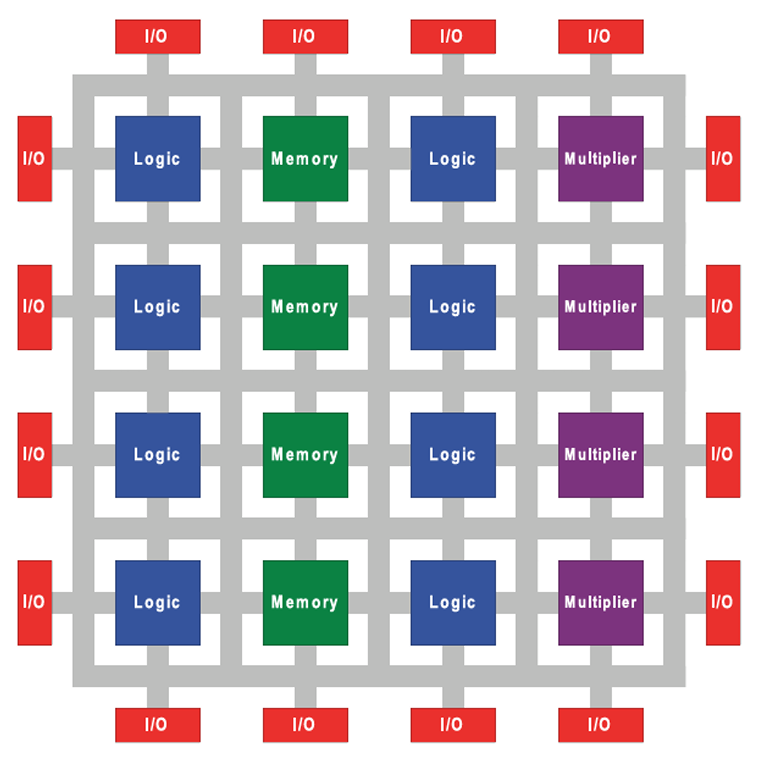
\includegraphics[width=0.6\linewidth]{pics/Uno.png} 
    \caption{Diagrama simplificado de matriz de programable de compuertas lógicas. \cite{kuon2007fpga}}
    \label{fig:Uno} 
\end{figure}

\subsection{Tablas de Consulta}

Las tablas de consulta son la herramienta mediante la cual se genera la lógica en una
FPGA, en lugar de utilizar compuertas lógicas y tener que redirigir miles de compuertas
lógicas, lo que se utiliza son celdas de memoria en conjunto con multiplexores de esta
manera se genera una tabla de verdad dentro del sistema mediante un bitstream que lo
configura. También son conocidas como LUTs, según la cantidad de entradas se le añade
un número al final a modo de identificación, del número de entradas depende la cantidad
de bits de configuración que tiene una LUT en el caso de una LUT4 se tienen 16 posiciones
de memoria para cada una de las cuatro entradas y para la salida, en el caso de una LUT6
se tiene 64 bits de configuración. Aunque las LUTs sean escalables es importante analizar
las consecuencias de su escalabilidad, ya que existe una curva que describe los cambios en
el área y cantidad de LUTs en cierto área.
\cite{hassani2024efficient, kuon2007fpga, meyerbaese2014digital} 

En la figura 2.2 se muestra que el punto óptimo del tamaño de las LUTs se encuentra cerca
de LUT5, no obstante, se aclara que esto no impide tener LUT6 aunque solo se cuente
con LUT5, debido a que se va a trabajar con conglomerados de LUTs estos se pueden
conectar en paralelo para crear LUTs modulares que representen un LUT6, a forma de
ejemplo los LUT5 tienen 32 posiciones de memoria y los LUT6 tienen 64 posiciones de
memoria, por lo que al utilizar dos LUT5 se puede generar la lógica necesaria para un
LUT6. La práctica anterior es una eficiente solución para evitar el malgasto de área de la
FPGA enLUTs. Anivel de implementación física se suele utilizar SRAM para la memoria
de las LUTs y estos constituyen los bloques blandos de la FPGA.
\cite{kuon2007fpga, abderrahmaneMaximizeFlexibility}

\begin{figure}[h!]
    \centering 
    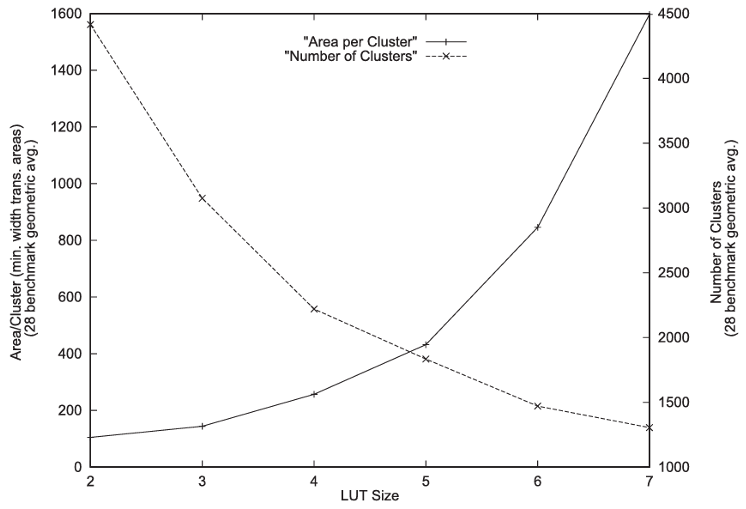
\includegraphics[width=0.7\linewidth]{pics/Dos.png} 
    \caption{Grafica de LUT de uso optimo. \cite{kuon2007fpga}}
    \label{fig:Dos} 
\end{figure}


Se debe tomar en cuenta para la eficiencia de una FPGA, no solo tiene lógica reconfigu
rable, también cuenta con módulos especializados, en el caso de que toda la lógica sea
reconfigurable, se pueden utilizar múltiples LUTs en algo que no es necesario por ejemplo
en bloques de multiplicación, este tipo de bloque es conocido como bloque rígido ya que
su función es fija. Su implementación es grabada sobre el propio silicio haciéndola no
reconfigurable, pero su ventaja se encuentra en su rendimiento ya que al estar sobre el
silicio funcionan de manera más rápida que una tabla de consulta y requiere poca área
del silicio.
\cite{kuon2007fpga, meyerbaese2014digital, abderrahmaneMaximizeFlexibility}

\subsection{Enrutamiento}

La arquitectura del enrutamiento en una FPGA es lo que da conexión a las LUTs al
igual que sus entradas, salidas y los bloques rígidos para completar la lógica diseñada. La
arquitectura utilizada es la arquitectura tipo isla como se muestra en la figura 2.3. En
dicha arquitectura se tienen los bloques lógicos y canales de enrutamiento a los cuatro
lados de dichos bloques lógicos, la cantidad n de cables que contiene un canal se define
durante la fabricación, sin embargo, es de los parámetros más importantes que puede
tener una FPGA ya que define la cantidad de señales que se pueden trabajar de manera
simultánea.
\cite{hassani2024efficient, kuon2007fpga} 

\begin{figure}[h!]
    \centering 
    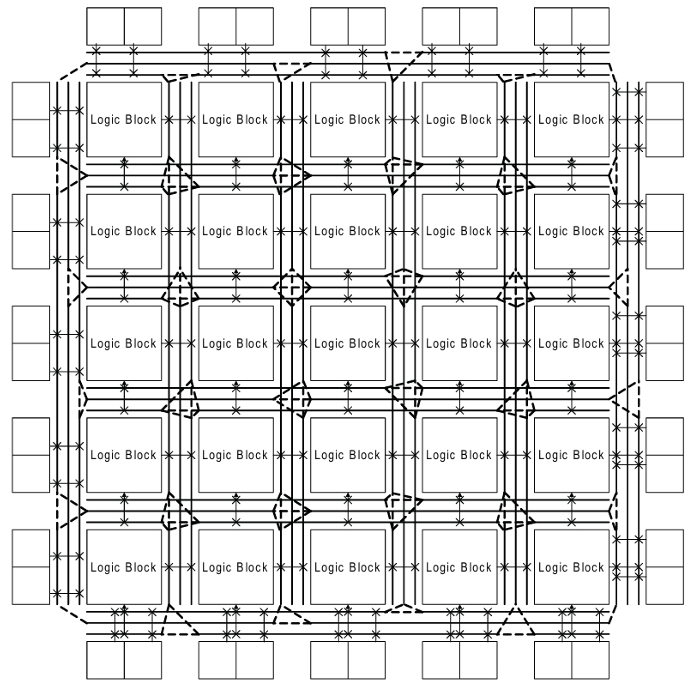
\includegraphics[width=0.6\linewidth]{pics/Tres.png} 
    \caption{Diagrama de configuración del enrutamiento y bloques lógicos. \cite{kuon2007fpga}}
    \label{fig:Tres} 
\end{figure}


La lógica de la arquitectura de isla se basa en dos sencillos términos, cables largos y
cables cortos, los cables largos componen los canales que se observan en paralelo a los
bloques lógicos, su principal función es ser una malla de interconexión entre las señales
que se generen o ingresen a la FPGA. Los cables cortos son el medio por el que las señales
entran a un bloque desde la malla de enrutamiento o por la que la señal sale de un bloque
a la malla de enrutamiento como se muestra en la figura 2.4.
 \cite{kuon2007fpga, meyerbaese2014digital} 

\begin{figure}[h!]
    \centering 
    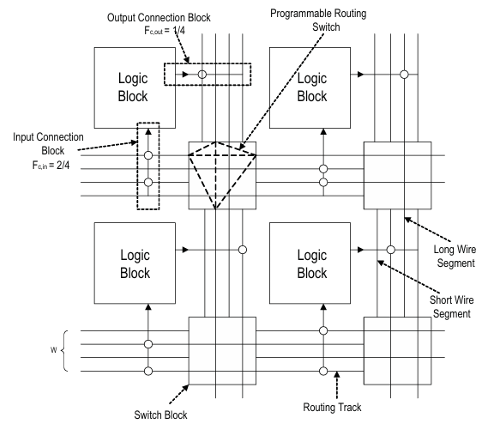
\includegraphics[width=0.6\linewidth]{pics/Cuatro.png} 
    \caption{Diagrama de bloques de cables cortos y largos. \cite{kuon2007fpga}}
    \label{fig:Cuatro} 
\end{figure}


Cabe mencionar que existen arquitecturas de enrutamiento que dependen del orden jerárquico 
para ordenar la transferencia de datos, pero a manera que la jerarquía aumenta, los
retardos aumentan de manera significativa perdiendo el sentido de que existan múltiples
niveles jerárquicos y haciendo esta arquitectura contraproducente al objetivo de flexibili
dad inherente de una FPGA. La malla de enrutamiento se encarga del desplazamiento de
datos en la arquitectura de una FPGA, no obstante, la gestión de los datos es responsa
bilidad de la matriz de conmutación.
\cite{hassani2024efficient, kuon2007fpga} 

\subsection{Matriz de conmutación}

La malla de enrutamiento conecta todos los bloques de la arquitectura, pero aún se deben
dirigir dichos datos, para que sean la entrada de un bloque o inclusive para que dos bloques
trabajen los datos en paralelo, la matriz de conmutación es el mecanismo mediante el cual
se ordenan las pistas de cables y se define a las señales cuál bloque es su próximo ingreso.
Estas rutas se definen desde que se carga el bitstream a la FPGA, por lo que las rutas
son flexibles previas al bitstream, pero estáticas una vez programadas. Su funcionamiento
se caracteriza por el uso de multiplexores para definir la ruta, sin embargo también se
implementa la lógica necesaria mediante transistores de paso para definir su ruta.
\cite{hassani2024efficient, kuon2007fpga} 

Se considera la intersección de dos canales como una matriz de conmutación, en dichos
canales donde cada cable interseca con otro cable se debe considerar la posibilidad de que
la señal viaje sobre el mismo cable en la misma dirección inicial, que siga una ruta ascen
dente por el cable con el que interseca, o una ruta descendente por el cable que interseca.
Para definir la ruta específica que se desea, se requieren de al menos seis transistores de
paso para aislar la ruta en el caso de que no se desee bifurcar la señal, las ubicaciones
específicas para dichos transistores de paso son conectando la sección de cable izquierdo
con el derecho, conectando la sección ascendente con la descendente, la izquierda con la
ascendente, la izquierda con la descendente, la ascendente con la derecha y la descendente
con la derecha, de esta manera se tiene un control total sobre la dirección deseada de la
señal, su control se basa en los datos guardados en una memoria SRAM que requiere seis
bits de control, considerando un bit por transistor de paso y una SRAM por intersección
de los cables largos tal y como se muestra en la figura número.
\cite{hassani2024efficient, kuon2007fpga} 

\begin{figure}[h!]
    \centering 
    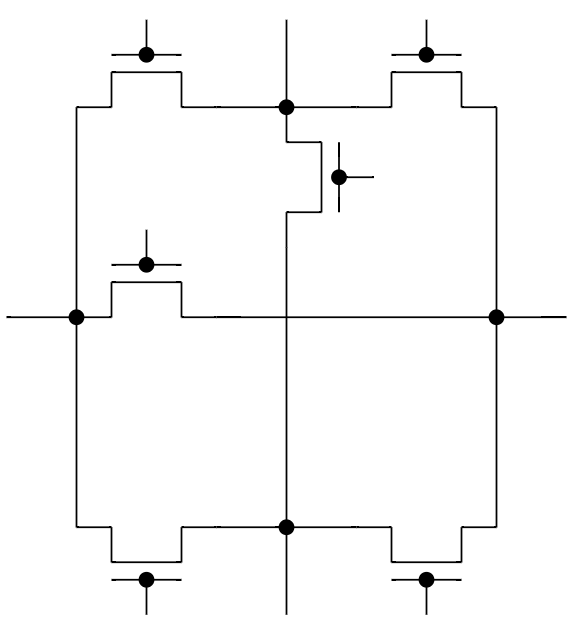
\includegraphics[width=0.4\linewidth]{pics/Cinco.png} 
    \caption{Diagrama matriz de conmutación.  \cite{kuon2007fpga}}
    \label{fig:Cinco} 
\end{figure}

\section{Arquitectura Modulo de Jerarquía Superior}

Considerando el funcionamiento de una FPGA, es necesario tener un conocimiento del
proceso entre el diseño y la descripción de hardware, para cualquier sistema, esto debido
al flujo de bits necesario para dar propósito a la FPGA. Se debe implementar un inyector
del flujo de bits además de la FPGA embebida en el nivel superior de jerarquía, de otra
manera la FPGA embebida se mantiene en un estado sin programar. Se requiere algún tipo
de memoria que se pueda utilizar para luego serializar y cargarla a la FPGA embebida.
Las ROM cumplen con características específicas para probar el funcionamiento de la FP
GAembebida en conjunto con lógica secuencial que permite la serialización de los datos de
la ROM para su posterior inyección en el sistema, de esta implementación suele encargarse
el software de diseño en conjunto con los puertos del hardware para la configuración.
\cite{hassani2024efficient, kuon2007fpga, meyerbaese2014digital} 

\subsection{Escaneo de Fronteras/JTAG}
El Joint Test Action Group, fue desarrollado para resolver problemas en el área de testing 
de circuitos integrados, esto debido a que los circuitos integrados cada vez disminuían el 
tamaño y los pines de prueba que se utilizaban acaparaban mucha área del circuito integrado 
por lo que se investigaban nuevos métodos de probar la funcionalidad de los circuitos 
integrados. El estándar IEEE 1149.1 surge en 1990 y define la arquitectura TAP en conjunto 
con el JTAG para diagnóstico, manufactura, validación, caracterización y debug de los 
circuitos integrados. 
\cite{nelsonBoundaryScan, calvoTestingSesion4, xjtagWhatIsJtag, jtagTechnologiesBoundaryScan, jtagTechnologiesTapController, ieee1149}

\begin{figure}[h!]
    \centering 
    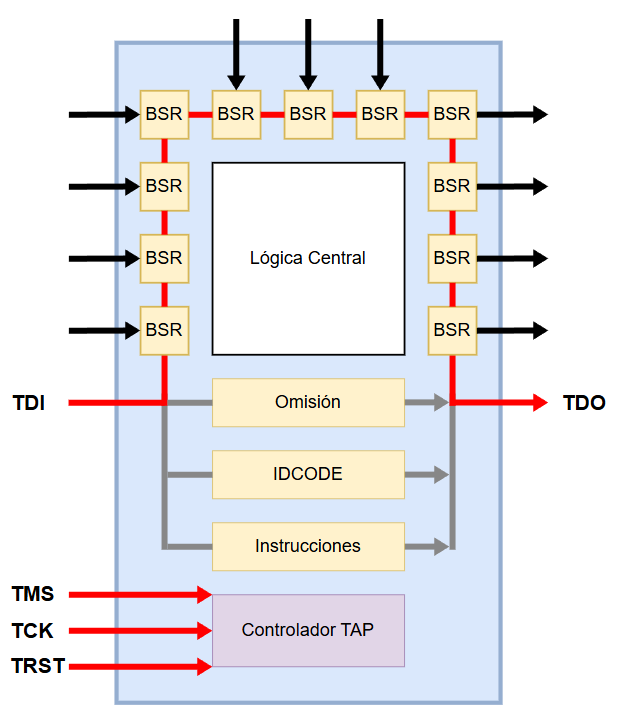
\includegraphics[width=0.4\linewidth]{pics/Seis.png} 
    \caption{Diagrama de la arquitectura TAP. \cite{jtagTechnologiesBoundaryScan}}
    \label{fig:Seis} 
\end{figure}

\subsection{Interfaz del Puerto de Acceso de Prueba}

Su conexión física se basa en 4 pines, TDI (Entrada de datos serial), TMS (Control), TCK (Reloj), 
TDO (Salida de datos serial) y en ocasiones se añade un pin extra TRST (Reinicio asíncrónico), estas cuatro o 
cinco señales son conocidas como TAP (Puertos de acceso para pruebas). En el contexto de las 
FPGAs , se utiliza el JTAG para acceder a la configuración de la memoria para programar el 
dispositivo, para visualizar la lógica programable del núcleo y el ruteo de los recursos. 
Esto se ejemplifica en las secciones pasadas dedicadas a explicar la arquitectura de lógica 
reconfigurable de las FPGAs, donde los registros SRAM configuran las tablas de búsqueda, los 
caminos que deben seguir los recursos y la disposición de la matrices de conmutación.
\cite{nelsonBoundaryScan, calvoTestingSesion4, jtagTechnologiesBoundaryScan, jtagTechnologiesTapController} \cite{ieee1149}

\begin{figure}[h!]
    \centering 
    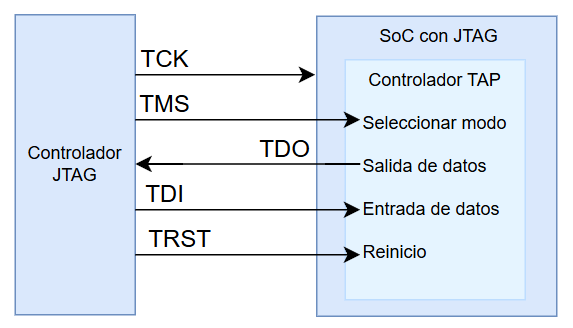
\includegraphics[width=0.6\linewidth]{pics/Siete.png} 
    \caption{Diagrama de conexion JTAG y TAP.  \cite{jtagTechnologiesTapController}}
    \label{fig:Siete} 
\end{figure}


\subsection{Controlador JTAG TAP}

El controlador TAP es el mecanismo de control base del estándar IEEE 1149.1, en este se 
define como los datos son ciclados a través del dispositivo y determina si se accede a alguno 
de los registris de datos e/o instruciones. Las señales del controlador se acceden mediante 
la interfaz TAP explicada anteriormente. El pin de mayor significado para el codntrolador TAP 
es el TMS debido a que es la entrada (un solo bit) de la máquina de estados que define el 
camino a tomar de los 16 estados existentes.
\cite{nelsonBoundaryScan, calvoTestingSesion4, jtagTechnologiesBoundaryScan, jtagTechnologiesTapController, ieee1149}

Al ordenar los estados en funcionalidad, se obtinen 3 subcategorías:
\begin{itemize}
    \item Prueba de lógica de reinicio y Marcha/Inactivo.
    \item Estados de accedo al registro de insrucciones (IR).
    \item Estados de acceso a los registros de datos (DR).
\end{itemize}
\cite{nelsonBoundaryScan, calvoTestingSesion4, jtagTechnologiesBoundaryScan, jtagTechnologiesTapController, ieee1149}

\begin{figure}[h!]
    \centering 
    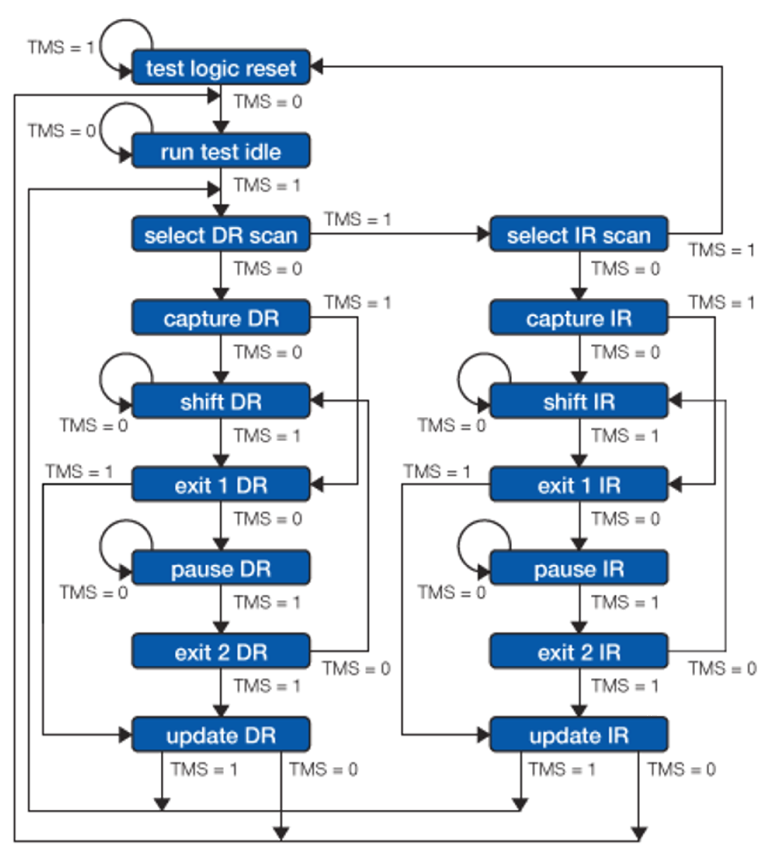
\includegraphics[width=0.6\linewidth]{pics/Ocho.png} 
    \caption{Máquina de estados del controlador TAP.  \cite{jtagTechnologiesTapController}}
    \label{fig:Ocho} 
\end{figure}

\subsection{Registros del JTAG}

El estándar IEEE 1149.1 define dos tipos de registros, los registros de datos y los registros 
de instrucciones. 
\cite{nelsonBoundaryScan, calvoTestingSesion4, jtagTechnologiesBoundaryScan, jtagTechnologiesTapController, ieee1149}

\subsubsection{Registros de datos}
Los registros de datos incluyen:

\begin{itemize}
    \item El registro de escaneo de frontera (BSR).
    \item El registro de omisión (BYPASS).
    \item El registro del código de identificación (IDCODE).
\end{itemize}

El controlador TAP se encarga de definir a cuál se accesa mediante la máquina de estados ya 
que solo se puede utilizar un registro de datos a la vez. 
\cite{nelsonBoundaryScan, calvoTestingSesion4, jtagTechnologiesBoundaryScan, jtagTechnologiesTapController, ieee1149}

El BSR no es un registro de un solo bloque, sino el una cadena de bloques que funcioan como 
registro de corrimiento para forzar valores a pines específicos internamente en el SoC, de 
igual manera se puede utilizar como un muestreo  de los valores de los pines considerando que 
son solo de lectura para realizar un censado.
\cite{nelsonBoundaryScan, calvoTestingSesion4, jtagTechnologiesBoundaryScan, jtagTechnologiesTapController, ieee1149}

El registro de omisión solo cuenta con un bit de logitud, y su función es habilitar o 
desconectar el uso del registro BSR, funciona como paso a la entrada de otros SoC que se 
quieren probar en serie con el primero, esto permite la optimización del flujo de bits.  
\cite{nelsonBoundaryScan, calvoTestingSesion4, jtagTechnologiesBoundaryScan, jtagTechnologiesTapController, ieee1149}

El registro del código de identificación es un registro de 32 bits que contiene la 
identificación única del dispositivo, está grabada en el silicio para evitar su modificación, 
sirve para que el software sea capaz de identificar el hardware y utilice valores correctos de 
tensión para el registro BSR y la correcta cantidad de bits.
\cite{nelsonBoundaryScan, calvoTestingSesion4, jtagTechnologiesBoundaryScan, jtagTechnologiesTapController, ieee1149}

\section{Filtrado digital}

Basado en la funcionalidad de la transformada discreta de Fourier como representación
finita en el dominio de la frecuencia. El filtro digital es un filtro matemático que realiza
una convolución, que matemáticamente se puede explicar secuencialmente como un des
plazamiento temporal, la multiplicación de la señal por otra señal de referencia y la suma
de los resultados para generar el muestreo de la salida. Los filtro digitales se dividen en
dos tipos:
\begin{itemize}

    \item Filtros digitales de respuesta finita al impulso: Estos filtros tienen una respuesta
finita al impulso, lo que significa que su salida se vuelve cero después de un número
finito de muestras. Son estables y tienen una fase lineal, lo que los hace ideales para
aplicaciones donde la distorsión de fase es un problema.\cite{proakis1996digital}

    \item Filtros digitales de respuesta infinita al impulso: Estos filtros tienen una respuesta
infinita al impulso, lo que significa que su salida no se vuelve cero después de un
número finito de muestras. Son más eficientes en términos de recursos computacio
nales, pero pueden ser inestables y tener una fase no lineal.\cite{proakis1996digital}

\end{itemize}

Un ejemplo de un tipo de filtro digital es el filtro de coseno alzado, utiliza como referencia
un coseno y su principal fortaleza es reducir la interferencia entre símbolosonfiabilidad de
la transmisión de datos. El filtro de coseno alzado se utiliza en sistemas de comunicación
digital donde los símbolos pueden superponerse debido a la dispersión del canal.
\cite{proakis1996digital}

\section{Estado del Arte}

\subsection{eFPGAs}

El concepto de una FPGA embebida no es nuevo, las FPGAs se utilizan como solución an
tes piezas de hardware caras cuyo diseño no es complejo a nivel de características como la
potencia requerida o almacenamiento significativo. Su uso se encuentra incluso vinculado
a ASICs ya que también significa ahorro para los productores de dicho ASIC, no obstante,
en casos de eFPGAs en ASICs, las eFPGAs cuentan con características específicas para
la pieza de hardware que se desea implementar en conjunto con el ASIC, por lo que no se
espera una gran cantidad de tablas de consulta, menores velocidades de reloj para lógica
secuencial, e incluso puede que no se cuente con bloques rígidos especializados a menos
que el ASIC lo requiera. Algunos ejemplos de empresas a continuación.\cite{saidi2018survey}

Flex Logic es una compañía tecnológica que utiliza la tecnología de eFPGA desde el 2015,
los motiva la reutilización de un circuito integrado luego de su fabricación. Cuentan con
un núcleo de eFPGA conocido como FLX10 con 5-7 capas de metal, sus características
principales son:

\begin{itemize}

    \item 20K bits de RAM
    \item 122500 LUTs 6
    \item Coarse Grain
    
\end{itemize}

Mental trabaja con eFPGA desde el 2009, al igual que Flex Logic su objetivo es la
modificación de hardware post producción. La eFPGA de Menta cuenta con sus propias
herramientas para la compilación, diseño en RTL y configuración del eFPGA llamada
Origami.\cite{saidi2018survey}

\begin{itemize}

    \item 200000 LUTs 4
    \item Fine Grain
    
\end{itemize}

Achronix trabaja con eFPGA desde el 2016 su modelo de Speedcore eFPGA inlcuye
bloques de RAM, y bloques de procesamiento de señales digitales. Cuenta con el software
ACE para el diseño de herramientas, su principal uso es como acelerador de hardware y
coprocesador reconfigurable.\cite{saidi2018survey}

\begin{itemize}

    \item 1000 LUTs
    \item Coarse Grain
    
\end{itemize}

NanoXplore es una compañía que data del 2014 cuenta con la eFPGA NX-eFPGA que
se puede configurar mediante la aplicación NanoXmap para sintetizar RTL hasta el flujo
de bits, el uso de tablas de consulta de 4 entradas le permite utilizar menor área para la
eFPGA en la ASIC predeterminada.\cite{saidi2018survey}

\begin{itemize}

    \item 750000 LUTs
    \item Coarse Grain
    
\end{itemize}

La academia también presenta varias arquitecturas de eFPGA entre ellas:

\begin{itemize}
    \item FASE eFPGA
    \item EFPGA Based on Multistage Switching Networks
    \item ACLBs eFPGA
    \item Overlay eFPGA
    \item EFPGAs based on a flexible architecture
    \item ESL Re-programmable eFPGA
    \item EFPGA Subsystem
    \item LIP6 eFPGA
    \item FlexTiles
\end{itemize}

No se detallan sus características debido a que la mayoría utiliza LUTs de entre 4 y
6 entradas. Su uso es similar, sustituir una ASIC costosa en la implementación de un
proyecto o para investigación de su desarrollo.\cite{saidi2018survey}

\subsection{Herramientas de software}

FABulous es un generador de FPGA de código libre que implementa herramientas como
Yosys y nextpnr para el flujo de diseño, cuenta con la licencia Apache 2.0 para uso
comercial y académico. Cuenta con cierre del diseño de TSMC de 180nm, Skywater dde
130nm, IHP SG13G2, GF180MCU y 28nm CMOS.\cite{fabulous2024}

Yosys es una herramienta de código abierto para síntesis de Verilog RTL, tiene la licencia
ISC.\cite{wolf2024yosys}

\begin{itemize}

    \item Procesa casi cualquier diseño sintetizable en Verilog-2005.
    \item Mapeo a librerías de celdas estándar para ASICs.
    \item Mapeo para FPGAs Xilinx Serie 7 y Lattice iCE40 y ECP5.
    
\end{itemize}

Openlane es un traductor de RTL a GDSII basado en múltiples componentes como Yosys,
Magic, Netgen, CVC, SPEF-Extractor, Kayout entre otros, y es de código abierto. \cite{openlane}

%%%%%%%%%%%%%%%%%
  %\include{teoria}
  \chapter{Solución Propuesta}
\label{ch:solucion}

Este proyecto propone el desarrollo de una metodología de emulación física y caracterización para 
superar las limitaciones del hardware cerrado y disminuir los riesgos de la fabricación en 
silicio sin el previo modelado del sistema necesario. Para esto, se proponen cuatro etapas 
para la solución.

\section{Primera Etapa}

La primera etapa de la solución propuesta para el proyecto se enfoca en la selección de 
una arquitectura de lógica reconfigurable de código abierto parametrizable, y su 
implementación mediante un banco de pruebas para comprobar su funcionamiento correcto. De 
esta manera se elimina la dependencia del flujo de herramientas de un fabricante específico 
y se asegura la portabilidad del proyecto a diferentes plataformas, al igual que se garantiza 
la continuidad del proyecto en el caso de querer profundizar en el futuro.

\section{Segunda Etapa}

La segunda parte de la solución propuesta para el proyecto se centra en la instanciación de 
la arquitectura de lógica reconfigurable seleccionada en la primera etapa sobre una FPGA 
comercial. Mediante esta etapa se busca un medio para extraer en próximas etapas las métricas 
de rendimiento y uso de recursos como el área equivalente, el consumo de potencia y los 
retardos de las rutas críticas.

\section{Tercera Etapa}

La tercera fase de la solución propuesta para el proyecto busca implementar dos circuitos 
digitales que estresen la arquitectura de lógica reconfigurable seleccionada en la primera 
etapa de maneras diferentes. Para esto se propone la implementación de un filtro digital 
de orden bajo y un multiplicador de enteros. De esta manera se busca obtener métricas de 
rendimiento para su comparación y se garantiza la funcionalidad del flujo de síntesis y 
ruteo de la arquitectura de lógica reconfigurable seleccionada.

\section{Cuarta Etapa}

La cuarta etapa de la solución propuesta para el proyecto tiene como objetivo la consolidación 
de los datos obtenidos en la tercera etapa observando cómo las métricas de rendimiento se 
compensan entre sí, para determinar si la arquitectura de lógica reconfigurable seleccionada 
es adecuada para su uso en aplicaciones de alto rendimiento o si es necesario realizar 
modificaciones según la aplicación en la que se utilice. Esta etapa se enfoca en la 
interpretación de los datos y cómo su análisis puede guiar el diseño de futuras arquitecturas 
de lógica reconfigurable para su impresión en silicio.
  \chapter{Hipótesis y Objetivos del Proyecto}
\label{ch:HyO}

En este capítulo se presenta la base de la investigación: la hipótesis y las 
interrogantes derivadas de la misma. El objetivo general consiste en validar 
esta premisa, para lo cual se han definido objetivos específicos que abordan 
diferentes aspectos del tema. Asimismo, se describen las tareas precisas 
requeridas para alcanzar cada objetivo y lograr resultados concluyentes. Por 
último, se exponen las limitaciones del estudio.

\section{Hipótesis}
     ``La variación sistemática de los parámetros estructurales en una arquitectura 
     reconfigurable de hardware abierto permite identificar una configuración 
     óptima que maximiza el rendimiento de temporización para un conjunto específico 
     de circuitos benchmark, demostrando que la arquitectura de la red de 
     interconexión es el factor dominante en el consumo de potencia y área 
     sobre los bloques lógicos."
\section{Objetivos}

\subsection{General}
            Evaluar el impacto de la variación de parámetros estructurales en el 
            rendimiento, área y potencia de una arquitectura abierta de lógica 
            reconfigurable a nivel de simulación y pruebas físicas utilizando una 
            FPGA comercial como plataforma de emulación física.
\subsection{Específicos}
	\begin{itemize}
                \item Seleccionar una arquitectura de lógica reconfigurable de hardware 
                abierto y su flujo de herramientas asociado, justificando la elección 
                basado en su nivel de parametrización, soporte de verificación funcional 
                e historial de implementación física en otros proyectos.

                \item Configurar e instanciar la arquitectura seleccionada en una tarjeta 
                FPGA y caracterizarla basandose en reportes de síntesis, ruteo y ejecución 
                funcional, además de implementar al menos dos circuitos de prueba en dicha 
                lógica programable.
                             
                \item Caracterizar el impacto de la variación de los parámetros 
                estructurales disponibles en la arquitectura de lógica programable sobre 
                la utilización de recursos, el consumo de potencia y el rendimiento a nivel 
                de temporización.
    \end{itemize}
 
\section{Lista de Tareas por Objetivo}

Esta sección se enfoca en proporcionar un desglose detallado de las tareas que 
deben realizarse para lograr cada objetivo específico en el proyecto. Esta 
estructura por objetivo facilita la comprensión de las tareas individuales en el 
contexto de los objetivos más amplios del proyecto. Cada objetivo del proyecto 
tendrá su propia lista de tareas relacionadas, lo que proporciona una visión clara 
de lo que se debe lograr para alcanzar ese objetivo. Estas tareas se presentan de 
manera secuencial, lo que indica el orden en el que deben completarse.

\textbf{\normalsize{Objetivo Específico 1}}

Este objetivo se centra en la investigación de la arquitectura de 
lógica reconfigurable y el flujo de harramientas para su implementación, 
considerando la el soporte para su parametrización, verificación 
funcional e historial de implementación física.

\begin{enumerate}

    \item Investigar y recopilar información sobre las distintas 
    arquitecturas de lógica reconfigurable de hardware abierto 
    disponibles.
     
    \item Evaluar la flexibilidad y el nivel de parametrización 
    estructural que ofrece cada arquitectura preseleccionada.
    
    \item Analizar la madurez del flujo de herramientas asociado, 
    comprobando la compatibilidad y el soporte para la verificación 
    funcional.

    \item Revisar el historial de implementación física en silicio 
    de las opciones evaluadas para constatar su viabilidad y 
    confiabilidad en proyectos previos. 

    \item Seleccionar la arquitectura definitiva y justificar técnicamente 
    la elección, basada en el cumplimiento de los criterios previamente 
    analizados.

\end{enumerate}

Las tareas descritas justifican el uso de la arquitectura en las próximas 
etapas y su implementación en la FPGA.

\textbf{\normalsize{Objetivo Específico 2}}

El segundo objetivo se centra en la configuración de la arquitectura 
seleccionada mediante JTAG y la caracterización basada en reportes 
desplegados por las herramientas seleccionadas en la etapa anterior, 
además de la implementación de dos circuitos de prueba.

\begin{enumerate}

    \item Ajustar los módulos de la arquitectura seleccionada para asegurar 
    su compatibilidad con la herramienta de síntesis de la FPGA objetivo.
    
    \item Integrar la arquitectura en el proyecto principal de la herramienta de desarrollo.
    
    \item Correr el proceso de síntesis y extraer los reportes de la cantidad de LUTs, 
    flip-flops y bloques de memoria requeridos.

    \item Ejecutar la implementación en la FPGA y compilar los reportes de tiempos 
     de setup y hold, consumo de potencia estimado y congestión de ruteo.

    \item Generar el bitstream necesario para configurar la FPGA física.
    
    \item Seleccionar dos circuitos que estresen diferentes aspectos de la lógica programable.
    
    \item Codificar ambos circuitos independientemente.
    
    \item Escribir los testbenches correspondientes y simular el comportamiento 
    de los circuitos de prueba para asegurar su corrección funcional antes de la 
    implementación física.

    \item Compilar y cargar el primer y segundo circuito de prueba sobre la 
    arquitectura de lógica programable ya instanciada.

    \item Estimular las entradas en el hardware real, capturar las salidas y contrastar la 
    ejecución funcional contra los resultados obtenidos en las simulaciones

\end{enumerate}

Estas tareas permiten validar la arquitectura seleccionada y dan información benéfica para 
el desarrollo de la caracterización de la arquitectura seleccionada.

\textbf{\normalsize{Objetivo Específico 3}}

El tercer objetivo da base a la caracterizacion de la arquitecura de lógica programable 
seleccionada según la utilización de recursos.

\begin{enumerate}

    \item Identificar cuáles variables de la arquitectura de la arquitectura lógica 
    programable serán modificables.

    \item Definir un conjunto discreto de valores para cada parámetro seleccionado y 
    limitar las combinaciones posibles a un número manejable y representativo.
    
    \item Recopilar la cantidad de bloques lógicos básicos utilizados y la estimación de 
    área equivalente de silicio.

    \item Extraer del Análisis de Temporización Estática y el retardo de la ruta crítica.

    \item Compilar las estimaciones de consumo de potencia dinámica y estática reportadas 
    tras el ruteo.

    \item Procesar los datos consolidados para graficar el comportamiento de las métricas 
    frente a la variación de cada parámetro.

    \item Analizar los puntos donde la mejora de una métrica perjudica a otra (Trade-off).
    
    \item Concluir cuáles son las configuraciones de parámetros estructurales que ofrecen 
    el mejor balance técnico para los casos de uso proyectados.

\end{enumerate}


\section{Alcances y Limitaciones del Proyecto}

En la sección de limitaciones se exponen los desafíos y restricciones propios de la 
naturaleza del proyecto. Si bien estas condiciones pueden representar obstáculos, 
al mismo tiempo delimitan el alcance del trabajo y establecen un marco de referencia 
realista para su ejecución. A continuación, se detallan las principales limitaciones 
identificadas:

\begin{itemize}

    \item La ejecución de los experimentos se llevará a cabo con la FPGA 
    disponibles durante la evaluación del proyecto. Esta limitación en los recursos 
    físicos para la realización de pruebas podría restringir tanto la diversidad de 
    los escenarios evaluados como la naturaleza de los datos susceptibles de recolección.

    \item Al instanciar una arquitectura de lógica programable sobre una FPGA comercial, 
    el área, la potencia y el retardo de temporización estarán limitados por la arquitectura 
    de la FPGA anfitriona.

    \item La configuración óptima identificada estará restringida a las características 
    de los circuitos seleccionados y podría no ser generalizable a todas las aplicaciones 
    digitales.

    \item No se realizará una exploración exhaustiva de todo el espacio de diseño, por lo 
    que la configuración óptima que maximiza el rendimiento corresponderá únicamente a un 
    óptimo dentro del subconjunto explorado.

    \item Las métricas de consumo de potencia se extraerán a partir de reportes generados 
    por herramientas de síntesis y ruteo, no mediante mediciones físicas directas sobre 
    la arquitectura implementada por lo tanto se introduce un margen de error inherente a 
    los modelos matemáticos y estimaciones.



\end{itemize}
  \chapter{Experimento Preliminar}
\label{ch:Experimento}

En esta sección se especifica la estrategia planificada para realizar un 
experimento preliminar que permita validar la metodología propuesta para 
la emulación física y extracción de métricas de rendimiento en 
arquitecturas de lógica reconfigurable. Se escaló el experimento a un 
tamaño pequeño para asegurar su viabilidad en el tiempo del proyecto y 
su funcionamiento correcto, lo que permitirá realizar ajustes a la 
metodología antes de su aplicación a un sistema más complejo. El 
principal interés del experimento es garantizar la correcta síntesis, 
mapeo, reteo y generación del bitstream de la arquitectura lógica 
reconfigurable mediante un circuito digital de prueba básico sin 
intervención de hardware físico.

\section{Metodología del experimento}

Se diseñará mediante código RTL una microarquitectura de lógica 
programable por un solo grupo de cuatro tablas de búsqueda, 
matrices de conmutación y su ruteo respectivo, todo con sus registros 
para asegurar que sea reconfigurable.

Como circuito de referencia para emular dentro de la microarquitectura 
reconfigurable descrita, se utilizará un multiplexor de dos entradas, 
se describirá de manera estructural compuerta por compuerta como se 
muestra en la función lógica \ref{eq1}. Dicho multiplexor es compuesto 
por dos compuertas AND, una compuerta NOT y una compuerta OR, cada una 
de las compuertas será asignada a una de las LUTs disponibles en la 
microarquitectura reconfigurable.

\begin{equation}
	\label{eq1}
	Y = (A \cdot \overline{S}) + (B \cdot S)
\end{equation}

Fidnalmente se realizará una simulación funcional y de temporización 
utilizando un banco de pruebas en software para verificar que las 
señales de entrada conmuten correctamente hacia la salida según el 
estado de la línea de selección.

\section{Resultados Esperados}

Por este medio se pretende:

\begin{itemize}

	\item Confirmar que las herramientas abiertas son capaces de 
	reconocer la estructura de la microarquitectura reconfigurable y 
	mapear la lógica combinacional del multiplexor.

	\item Verificar que el software puede interconectar las LUTs de 
	manera exitosa para propagar la señal del multiplexor.

	\item Obtener los primeros reportes de retardo estimados por el 
	software, sirviendo como línea base para la metodología de 
	caracterización final.

\end{itemize}

  \chapter{Cronograma}
\label{ch:Crono}

En la Tabla  \ref{tabla:tareas} se muestra las actividades a desarrollar durante la investigación y elaboración del proyecto. La Figura 6.1 muestra el diagrama de Gantt correspondiente a las actividades.

\begin{table}[h]
\centering
\begin{tabular}{||c|l||}
\hline
\textbf{Tarea \#} & \textbf{Tarea a realizar} \\[1.5ex]
\hline\hline
1 & Investigación sobre las arquitecturas de lógica reconfigurable\\[1.5ex]
\hline
2 & Configuración del entorno de desarrollo y herramientas \\[1.5ex]
\hline
3 & Revisión y ajuste de los módulos en código RTL \\[1.5ex]
\hline
4 & Ejecución de los primeros procesos de síntesis lógica \\[1.5ex]
\hline
5 & Generación del archivo de configuración \\[1.5ex]
\hline
6 & Descripción de hardware de los dos circuitos de prueba \\[1.5ex]
\hline
7 & Procesamiento del filtro digital y el multiplicador de enteros \\[1.5ex]
\hline
8 & Extracción de las métricas finales \\[1.5ex]
\hline
9 & Análisis crítico de los puntos de trade-off  \\[1.5ex]
\hline
10 & Elaboración del informe escrito \\[1.5ex]
\hline
11 & Entrega del informe final \\[1.5ex]
\hline
12 & Defensa del proyecto \\[1.5ex]
\hline
\end{tabular}
\caption{Lista de tareas del proyecto}
\label{tabla:tareas}
\end{table}

\newpage

En la siguiente figura \ref{Gannt}, presentamos un Diagrama de Gantt que muestra gráficamente el cronograma de nuestro proyecto. Este diagrama nos permite visualizar con claridad la planificación de las diferentes actividades y su duración a lo largo de las semanas. Las tareas de cada objetivo específico están representadas por barras horizontales, cuya longitud es proporcional a la duración estimada de cada tarea. La organización de estas barras a lo largo de la línea temporal proporciona una perspectiva clara de cuándo y cómo se llevarán a cabo las actividades, facilitando así la gestión del tiempo y la distribución de los recursos. Las superposiciones indican la simultaneidad de tareas y las intersecciones demuestran los puntos donde las actividades están interconectadas. Este diagrama es la hoja de ruta visual de nuestro proyecto, y nos ayudará a mantenernos en la senda correcta, asegurando que todas las tareas se completen en los plazos establecidos.


         \begin{figure}[H]
		  \centering 
			  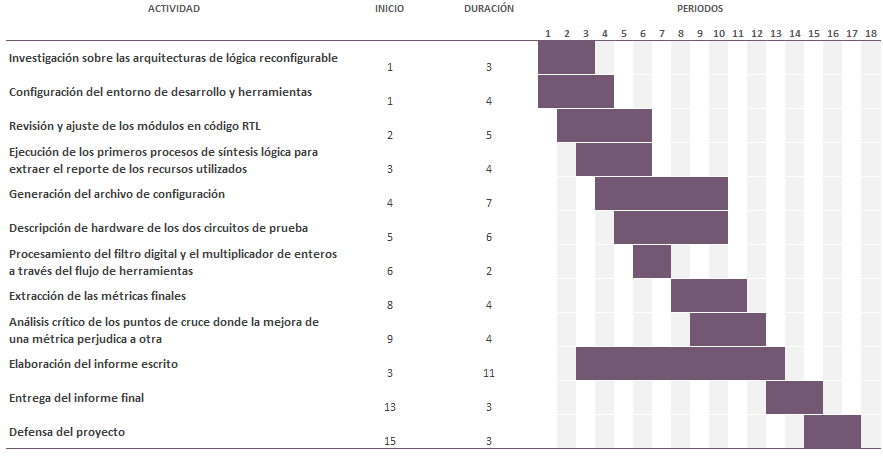
\includegraphics[scale=0.7]{pics/Cronograma.png}
			  \caption{Diagrama de Gantt de las actividades a realizar}
    		  \label{Gannt}
		\end{figure}



  %----------------------------------------------------------------------------
  % literature in bibtex way:
  % \bibliographystyle{sty/plainurl} % for english documents
  % \bibliography{literatura}
  % literature in biblatex/biber way
  % Ensure all entries from literatura.bib are included even if not cited
  \nocite{*}
  \printbibliography[title={Bibliografía},heading=bibintoc]
  %----------------------------------------------------------------------------

  %----------------------------------------------------------------------------
  \appendix
  %----------------------------------------------------------------------------

  %\chapter{Apendice}




  %----------------------------------------------------------------------------
  \backmatter
  %----------------------------------------------------------------------------

  \printindex                % insert index into document. Don't forget to call
                             % "makeindex filename" first.
                             
\end{document}